% March 2015
% Autor: Mandy Vogel
% getting started

\documentclass[xcolor={table},c]{beamer}
%\usetheme[backgroundimagefile=mathe]{diepen}
\usetheme{Frankfurt}
% \useoutertheme{miniframes}

%\setbeamerfont{block title}{size=\small,series=\bfseries}
%\setbeamerfont{block body}{size=\footnotesize}

% \usecolortheme{beetle}
\usepackage{linkimage}

%\usepackage{handoutWithNotes}
%\pgfpagesuselayout{3 on 1 with notes}[a4paper,border shrink=5mm]



\begin{document}
\title{Getting Started}   
\author{Mandy Vogel} 
\date{\today}

\AtBeginSection{
  \begin{frame}<beamer>{Table of Contents}
    \tableofcontents[currentsection]
  \end{frame}}

\begin{frame}
\titlepage
\end{frame}

\begin{frame}{Table of Contents}
\frametitle{Table of Contents}\tableofcontents
\end{frame}

\section{R}
\subsection{What is R?}

\begin{frame}\frametitle{What's R?}
  \begin{itemize}
    \item R is a high-level language and an environment for data analysis and graphics
    \item influenced by S (Becker, Chamber, Wilks) and Scheme (Sussman)
    \item and created by Ross Ihaka and Robert Gentleman at the university of Auckland
    \item R is free.
    \item R is open source.
    \item R is a dialect of S system.
  \end{itemize}
\end{frame}

\begin{frame}\frametitle{What R can do...}
  R provides a wide variety of statistical and graphical techniques including
  \begin{itemize}
    \item linear and nonlinear modelling
    \item classical statistical tests
    \item time-series analysis
    \item classification
    \item clustering and many more
  \end{itemize} \pause
    R is easily extensible, can produce publication-quality graphs including mathematical symbols; dynamic and interactive graphics are available through additional packages.
\end{frame}



\subsection{Why R?}
\begin{frame}\frametitle{Pros}
  \begin{itemize}
    \item R is free and R is open source
    \item there is a lot of material and books available
    \item there is a lot of help on the web, including developers who are active in mailing lists
    \item most of your problems are already solved and with a high probability the solution is available from one of the repositories (as package)
    \item there are a lot of intuitive GUIs
    \item the language is easy to learn and also intuitive
    \item the graphics capabilities are impressive
  \end{itemize}
\end{frame}


%% source for the next three slides: http://sites.google.com/site/r4statistics/popularity
\begin{frame}\frametitle{The number of analytics jobs for the more popular software (250 jobs or more, 2/2014).}
  \begin{center}
    \linkimage{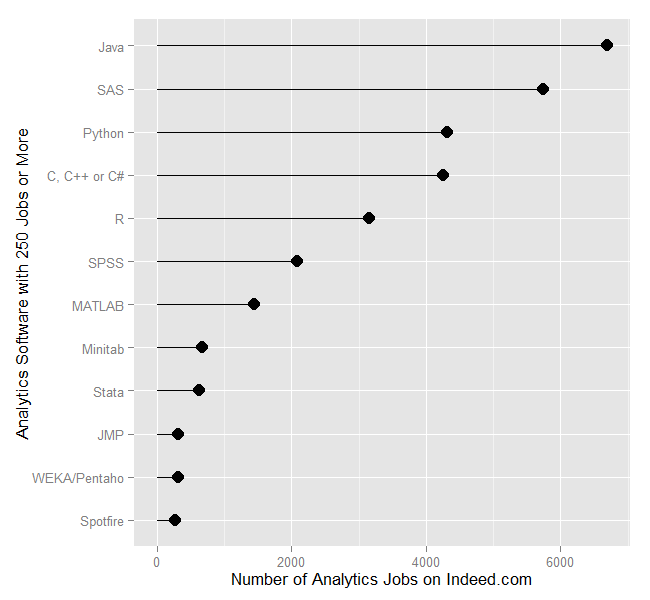
\includegraphics[width=8cm, height=6cm]{jobs.png}}{jobs.png}
  \end{center}
\end{frame}

\begin{frame}\frametitle{O’Reilly Data Science Survey results for 2012 and 2013 combined.}
  \begin{center}
    \linkimage{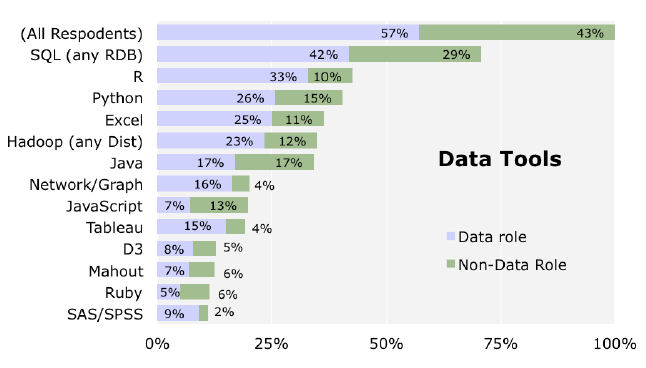
\includegraphics[width=8cm, height=6cm]{oreillystrata2013.png}}{oreillystrata2013.png}
  \end{center}
\end{frame}

\begin{frame}\frametitle{O’Reilly Data Science Survey results for 2012 and 2013 combined}
  \begin{center}
    \linkimage{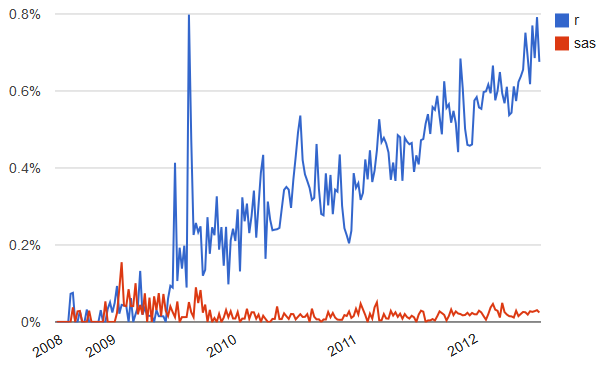
\includegraphics[width=8cm, height=6cm]{stackoverflowbyweek.png}}{stackoverflowbyweek.png}
  \end{center}
\end{frame}



\begin{frame}\frametitle{Cons}
  \begin{itemize}
    \item there is a LOT of help on the web
    \item with a high probability there is more than one solution for your problem
    \item there are a lot of intuitive GUIs so you have to decide what you want (so first you have to \emph{know} what you want)
    \item the real power of R (i.e. high flexibility) is not entirely available through GUIs
    \item and therefore the learning curve can be lengthy in the beginning (but soon accelerating ;)
  \end{itemize}
\end{frame}

\begin{frame}\frametitle{Use it!}
  The best way to learn R is to use it!
\begin{center}
 
\includegraphics[width=11cm]{user.png}
\end{center}
\end{frame}


\subsection{Getting R}
\begin{frame}[shrink=8,squeeze]{Where can I get it?}
  For the basic installation CRAN is a good place to start 
  \begin{itemize}
    \item CRAN stands for Comprehensive R Archive Network 
    \item \texttt{http://cran.r-project.org}\\ 
      \begin{itemize}
        \item Microsoft Windows: :: http://cran.r-project.org/bin/windows/base/\\
        \item  MacOS: :: http://cran.r-project.org/bin/macosx/\\
        \item  Linux: :: http://cran.r-project.org/bin/linux/\\ 
      \end{itemize}
    \item for mac and pc users: just download and install the precompiled binaries
    \item for ubuntu users: add \\ 
   \texttt{deb http://ftp5.gwdg.de/pub/misc/cran/bin/linux/ubuntu oneiric/} \\
to \\ \texttt{/etc/apt/sources.list}; \\ detailed howto: \\ \texttt{http://cran.r-project.org/bin/linux/ubuntu/} 
    \end{itemize}
\end{frame}

\begin{frame}\frametitle{The R-Commander}
The R commander, developed by John Fox is a complete GUI for R. It is implemented in the package \texttt{Rcmdr}:
\begin{itemize}
\item \texttt{Rcmdr} has a comprehensive menu, which includes data reading, summaries, statistical analyses, etc.
\item When the menu is activated, the \texttt{Rcmdr} will generate an R script. This script can be used as a log for documentation or for self learning.
\item It has excellent graphical tools.
\end{itemize}
\end{frame}

\begin{frame}\frametitle{The R-Commander}
\begin{columns}
  \begin{column}{0.5\textwidth}
    \begin{minipage}[c][4cm][c]{5.5cm}
      \linkimage{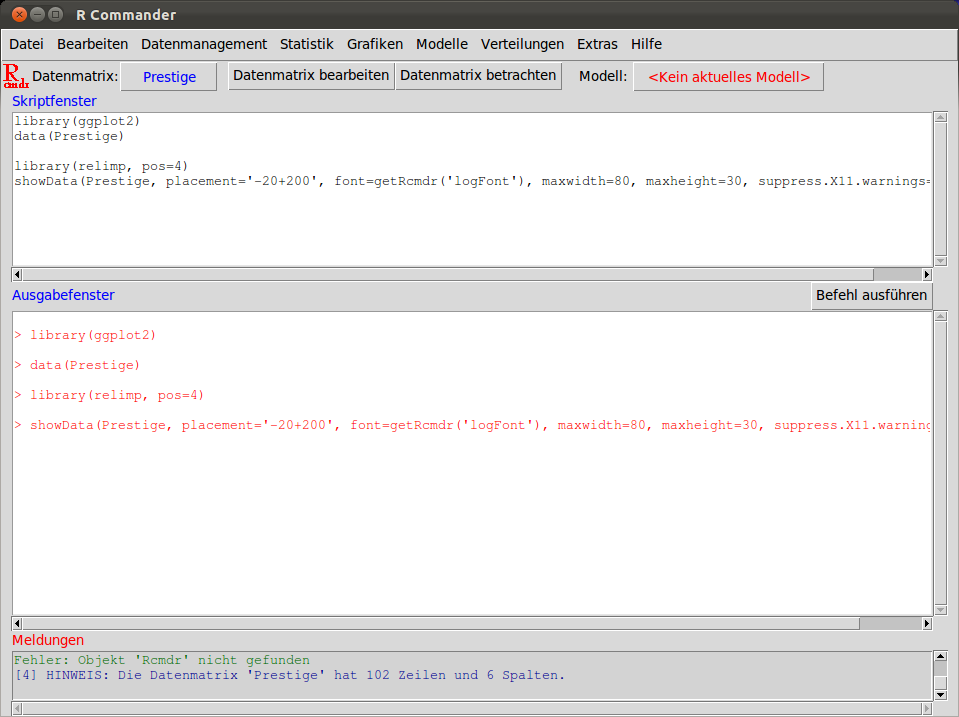
\includegraphics[width=5cm, height=3.5cm]{rcmdr.png}}{rcmdr.png}
    \end{minipage}
    \begin{minipage}[c][4cm][c]{5.5cm}
      \linkimage{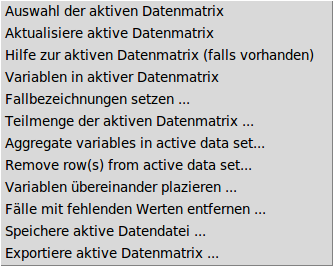
\includegraphics[width=5cm, height=3.5cm]{rcmdr3.png}}{rcmdr3.png}
    \end{minipage}
  \end{column}
  \begin{column}{0.5\textwidth}
    \begin{minipage}[c][4cm][c]{5.5cm}
      \linkimage{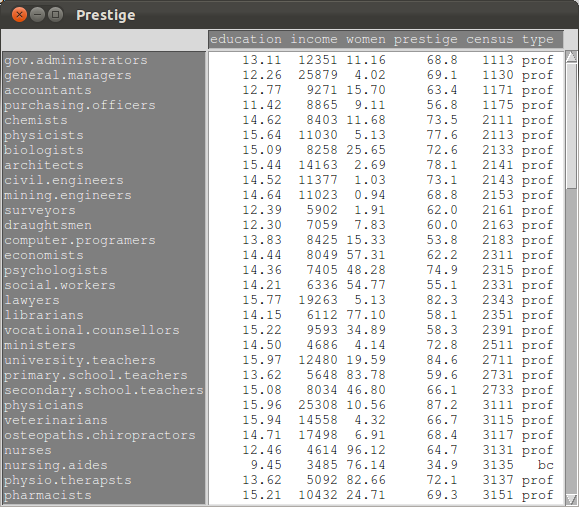
\includegraphics[width=5cm, height=3.5cm]{rcmdr2.png}}{rcmdr2.png}
    \end{minipage}
    \begin{minipage}[c][4cm][c]{5.5cm}
      \linkimage{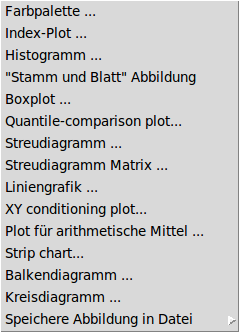
\includegraphics[width=5cm, height=3.5cm]{rcmdr4.png}}{rcmdr4.png}
    \end{minipage}
  \end{column}
\end{columns}
\end{frame}

\begin{frame}[fragile]\frametitle{The R-Commander}
To install \texttt{Rcmdr}  go to Packages $\rightarrow$ Install package(s) (or simply type \verb|install.packages("Rcmdr")|), then choose a CRAN mirror close to you, than OK. A window with a list of packages will pop-up, on this list choose \texttt{Rcmdr} and OK. A bundle of packages will be automatically installed.

To run the ''R Commander" GUI type at the prompt line:
\begin{verbatim}
> library(Rcmdr)
\end{verbatim}
This will start a GUI similar to other statistical software. Therefore, any typical process, like read data, produce plots, make statistical analyses, etc. will be made by clicking the appropriate menu.
\end{frame}

\section{RStudio}
\subsection{Installation}
\begin{frame}\frametitle{Getting R-Studio}
  RStudio is a free and open source integrated development environment (IDE) for R. You can run it on your desktop (Windows, Mac, or Linux) or even over the web using RStudio Server. Available at \texttt{http://rstudio.org/} (install R first)
\begin{center}
  \linkimage{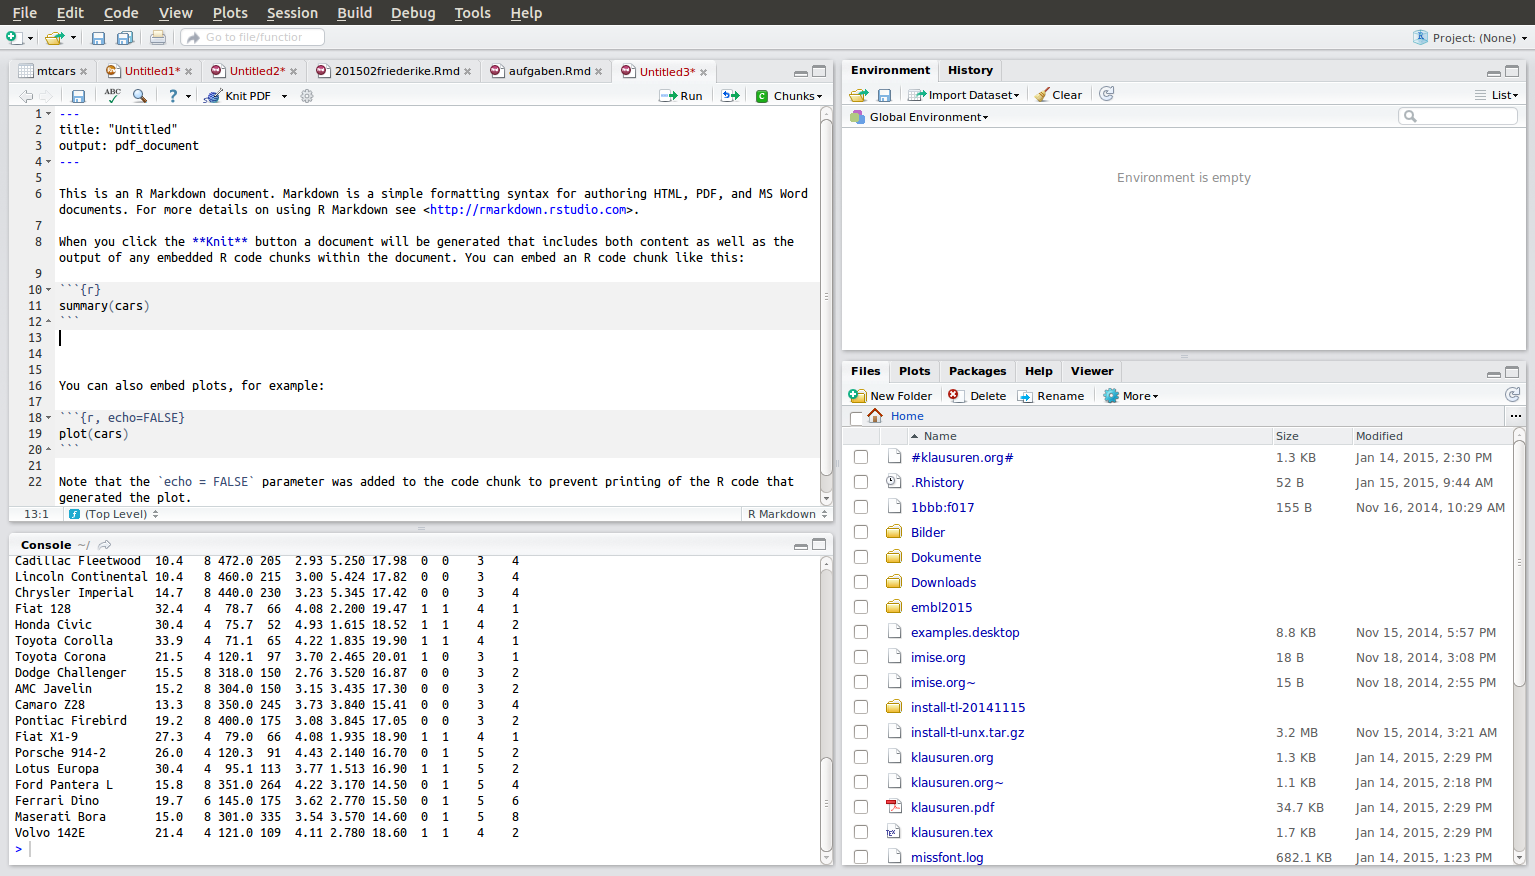
\includegraphics[width=5cm, height=4cm]{rstudio-ubuntu.png}}{rstudio-ubuntu.png}
\end{center}
\end{frame}

\subsection{Features}
\begin{frame}\frametitle{RStudio - Features}
  \begin{itemize}
  \item integration of the R console
  \end{itemize}
\begin{center}
  \linkimage{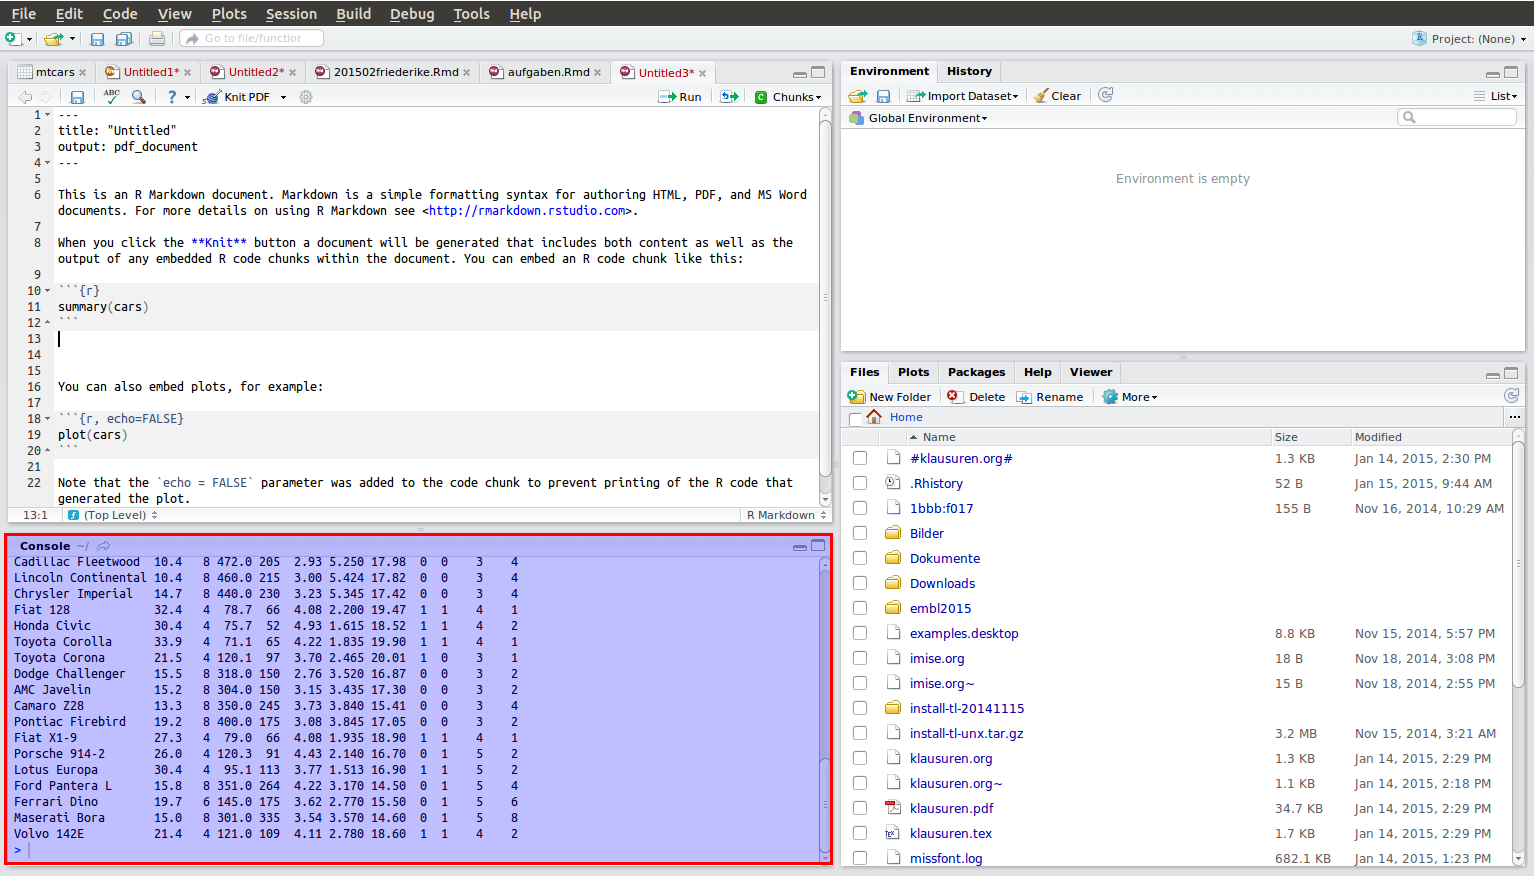
\includegraphics[width=6cm, height=4cm]{RStudioconsole.png}}{RStudioconsole.png}
\end{center}
\end{frame}

\begin{frame}\frametitle{RStudio - Features}
  \begin{itemize}
    \item code execution (Ctrl + Enter)
    \item different file types (mark down, c++, html, r)
    \item data viewer
  \end{itemize}
\begin{center}
  \linkimage{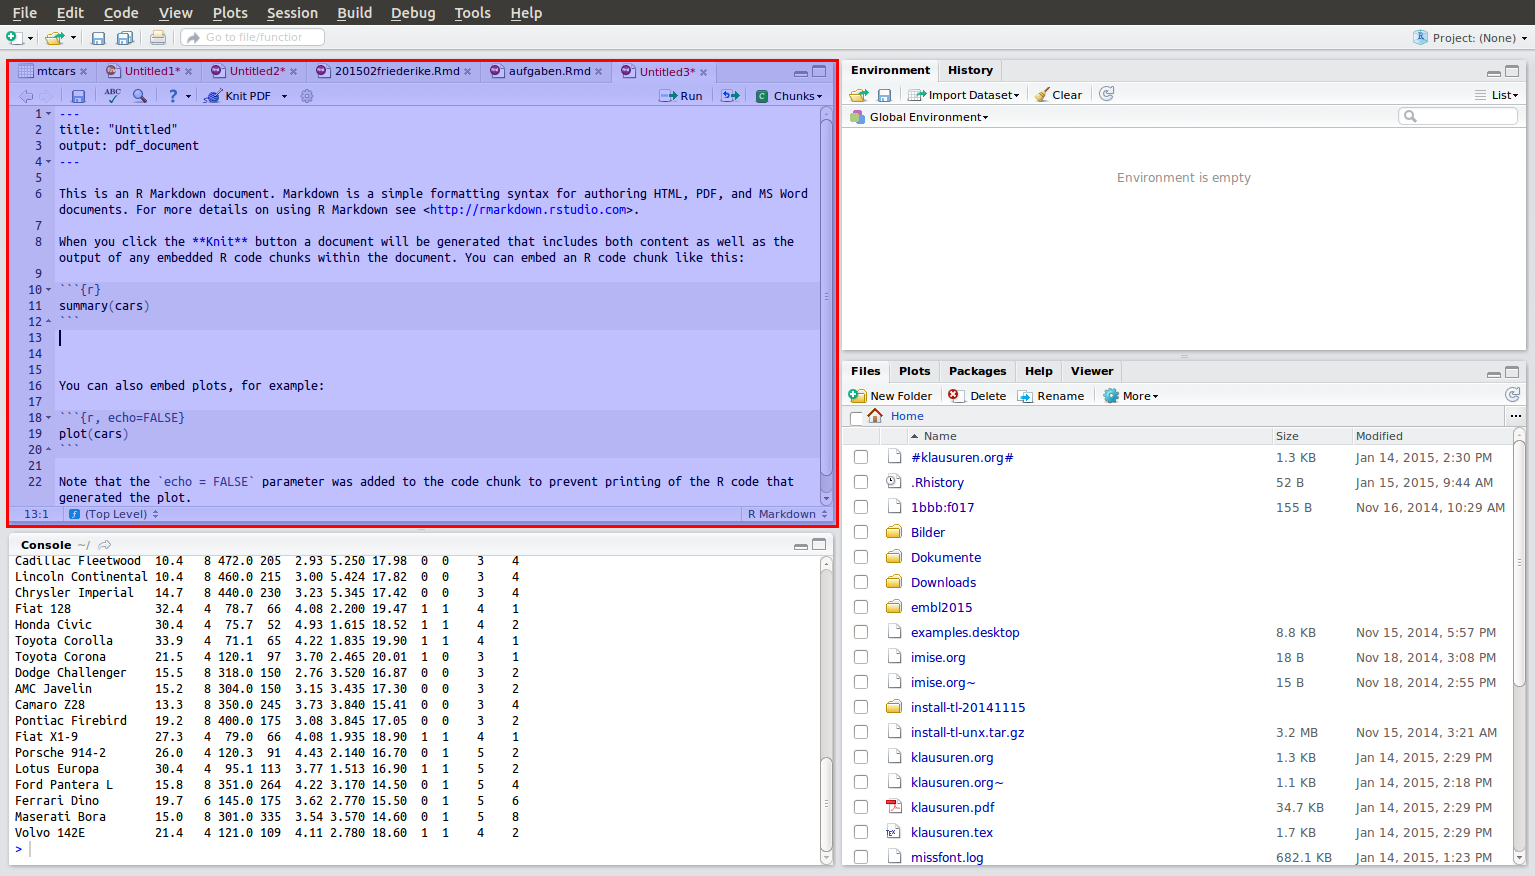
\includegraphics[width=6cm, height=4cm]{RStudioscript.png}}{RStudioscript.png}
\end{center}
\end{frame}

\begin{frame}\frametitle{RStudio - Features}
  \begin{itemize}
    \item syntax highlighting
    \item bracket support
    \item command completion (extensive use of the tab key is recommended)
  \end{itemize}
\begin{center}
  \linkimage{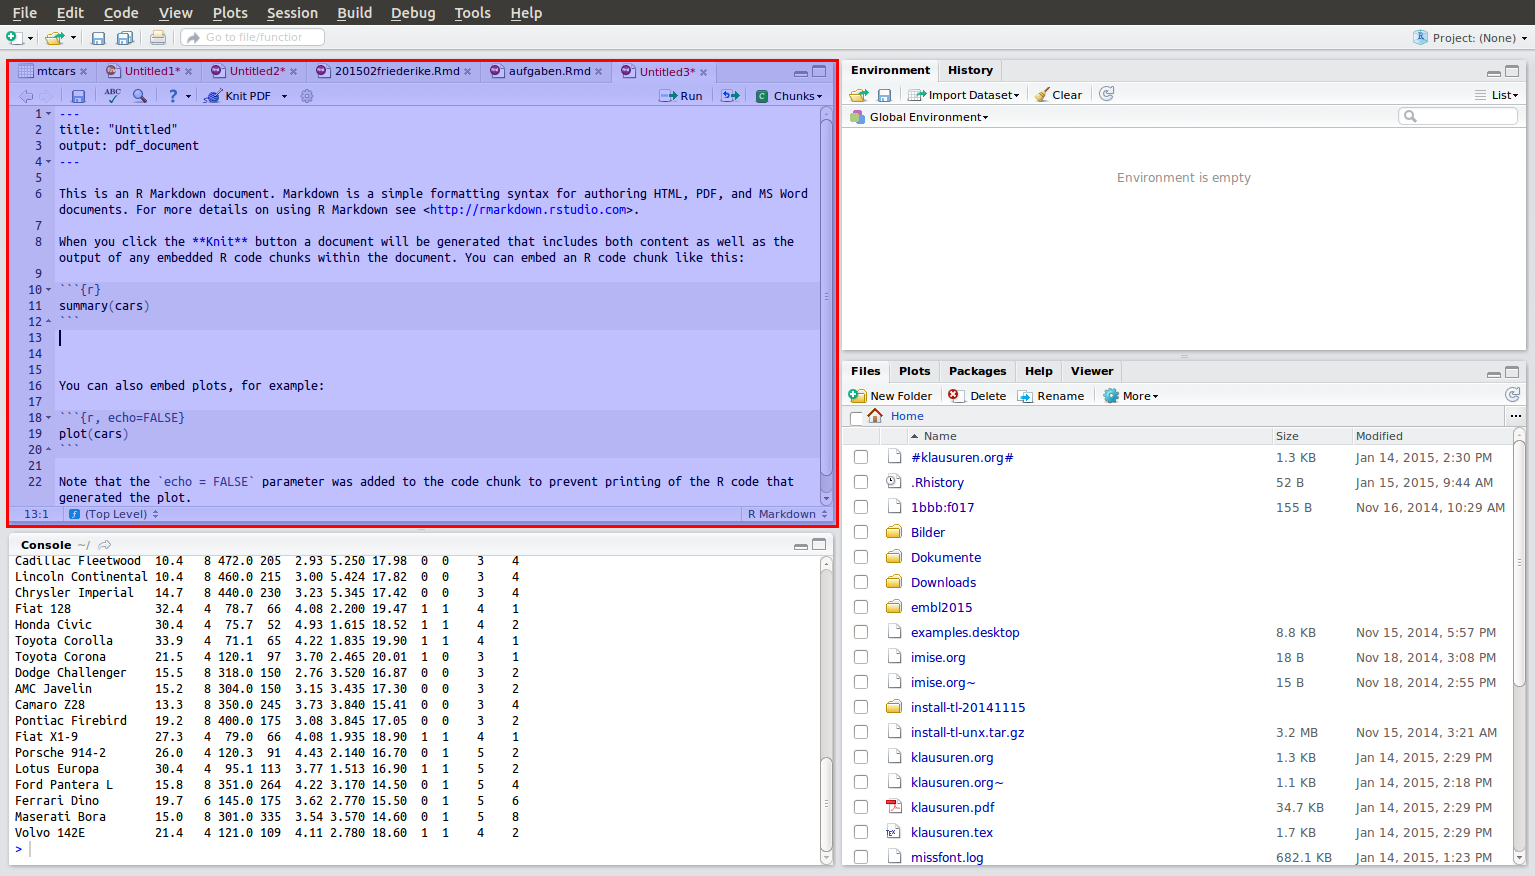
\includegraphics[width=6cm, height=4cm]{RStudioscript.png}}{RStudioscript.png}
\end{center}
\end{frame}


\begin{frame}\frametitle{RStudio - Features}
  \begin{itemize}
    \item object browser
    \item history browser
  \end{itemize}
\begin{center}
  \linkimage{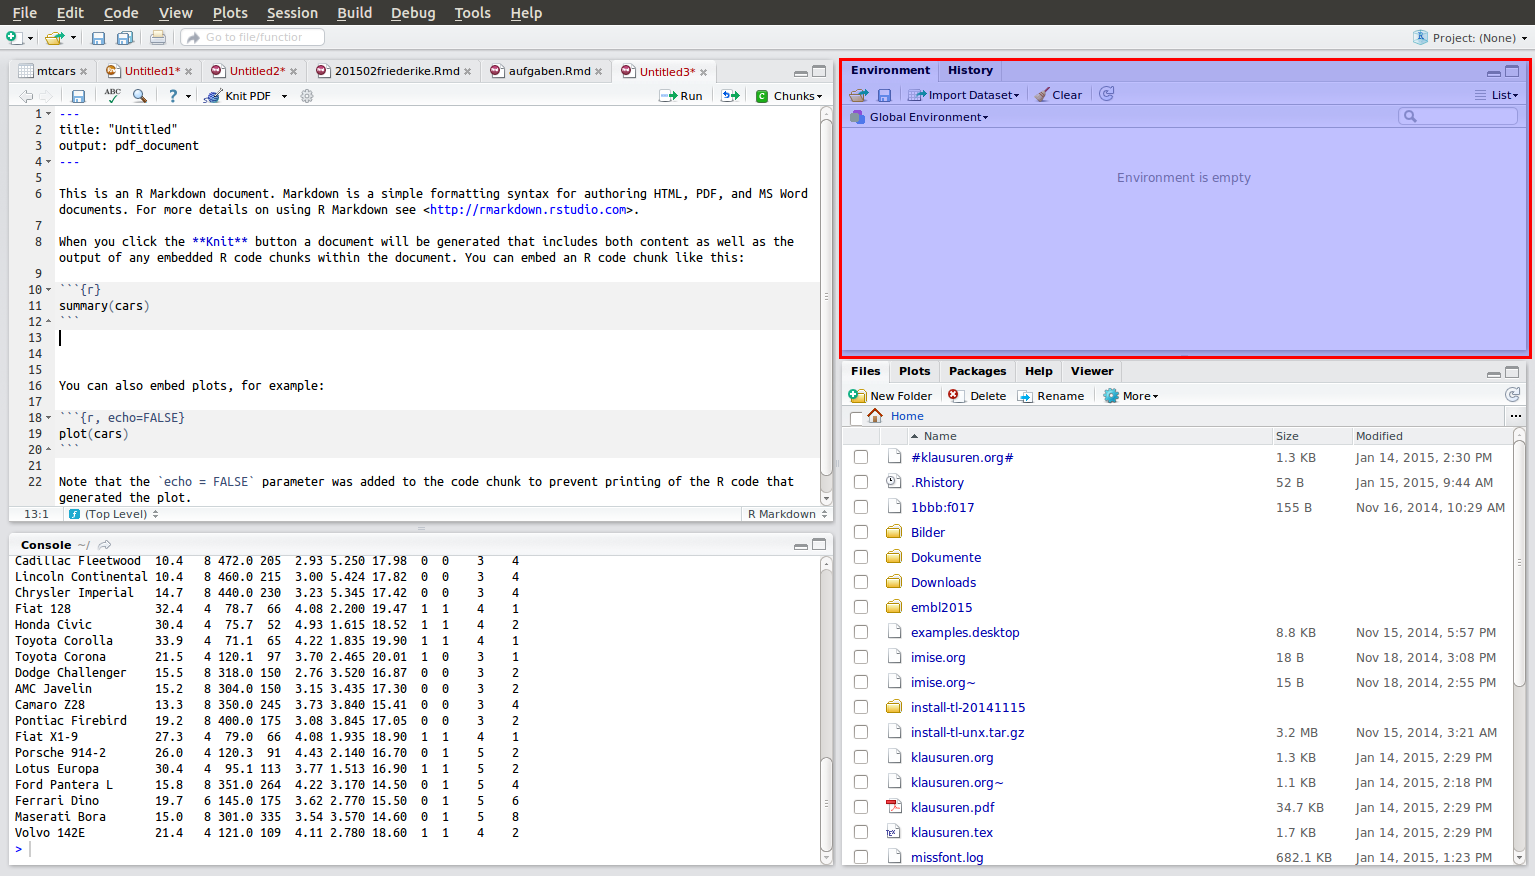
\includegraphics[width=6cm, height=4cm]{RStudioobjhist.png}}{RStudioobjhist.png}
\end{center}
\end{frame}


\begin{frame}\frametitle{RStudio - Features}
  \begin{itemize}
    \item file browser
    \item graphics integration
    \item help viewer
    \item package menu (installation, loading)
  \end{itemize}
\begin{center}
  \linkimage{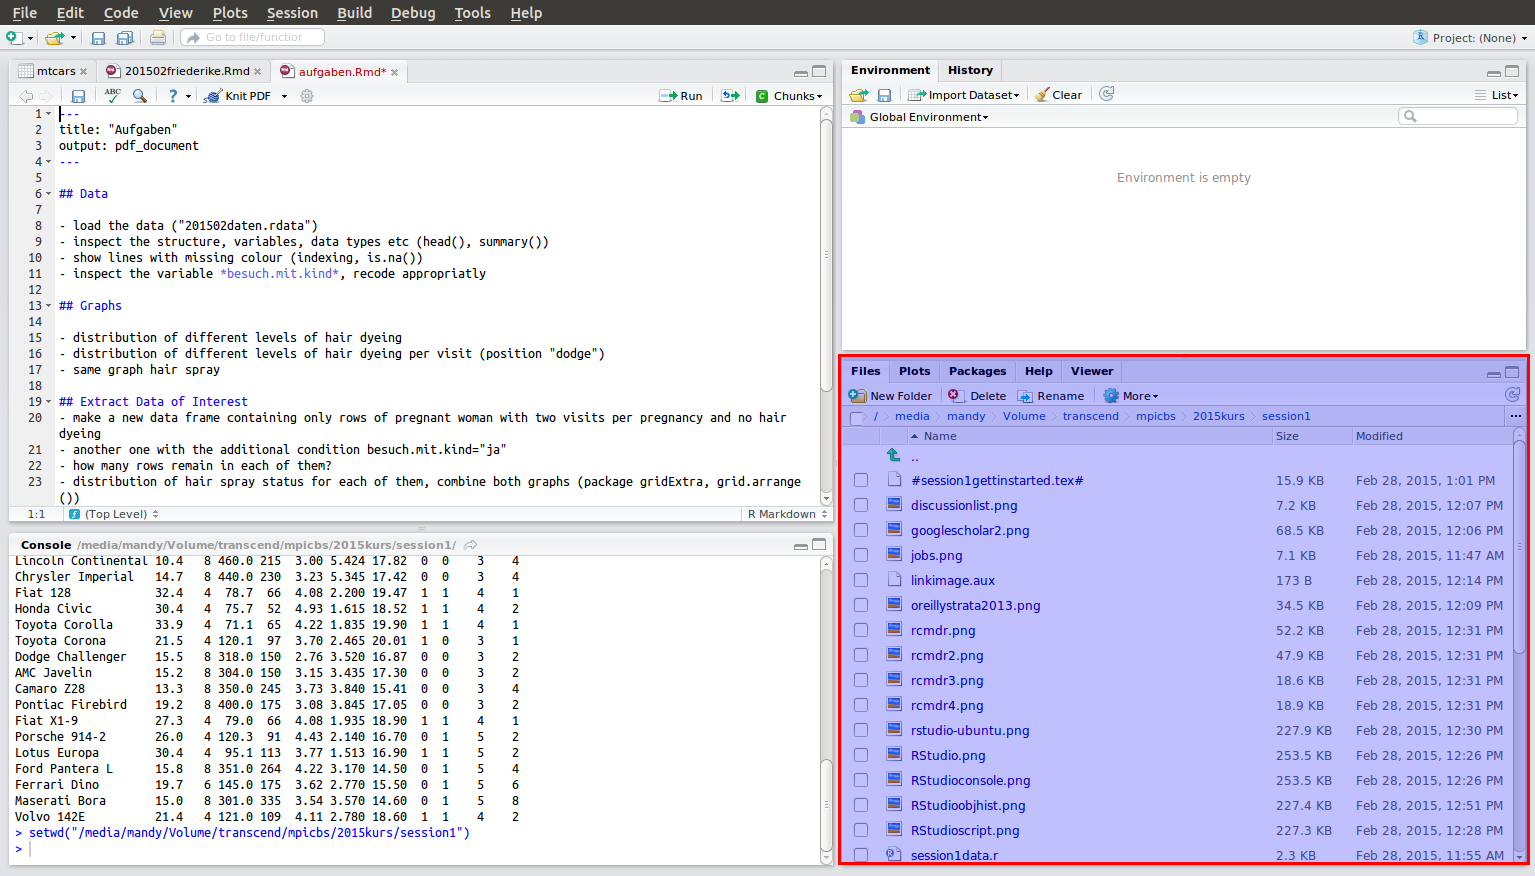
\includegraphics[width=6cm, height=4cm]{RStudiobottomright.png}}{RStudiobottomright.png}
\end{center}
\end{frame}



\section{Packages}
\subsection{What are packages for?}

\begin{frame}[shrink=5]\frametitle{Packages}
  The capabilities of R are extended through user-created packages, which allow specialized statistical techniques, graphical devices, import/export capabilities, reporting tools, etc. \newline

These packages are developed primarily in R, and sometimes in Java, C and Fortran. A core set of packages is included with the installation of R, with more than 6381 (as of Feb 2015) available at the Comprehensive R Archive Network (CRAN), 2095 (936 Software packages) on Bioconductor, and more on other repositories (e.g. R-Forge).
\begin{center}
  \linkimage{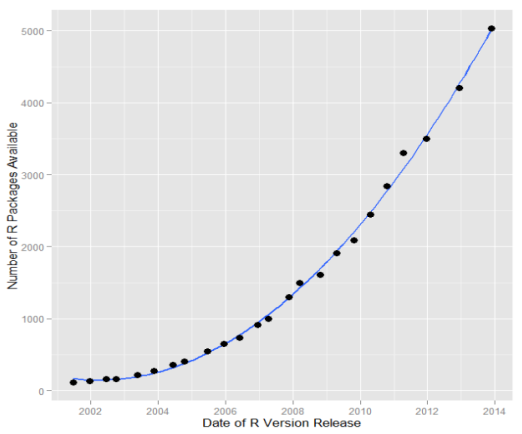
\includegraphics[width=6cm, height=4cm]{packages.png}}{packages.png}
\end{center}
\end{frame}

\subsection{How do I find the one I want}
\begin{frame}\frametitle{R taskviews}
  \begin{itemize}
    \item of course: you can google your problem: but you should use \texttt{http://www.rseek.org/} instead of \texttt{www.google.com}; \texttt{rseek} is a google custom search, can easily be added to the toolbar of popular browsers 
    \item \texttt{http://cran.r-project.org/web/views/}
    \item before you install a new package: \texttt{help.search()} allows for searching the help system for documentation matching a given character string in the (file) name, alias, title, concept
      or keyword entries (or any combination thereof), using either
      fuzzy matching or regular expression matching.(installed help system)
  \end{itemize}
\end{frame}

\begin{frame}[fragile]\frametitle{Packages}
  \begin{itemize}
  \item An R installation contains a library of packages. Some of these packages are part of the basic installation. These packages have the \emph{ recommended } status.
  \item Others (over 6000) can be downloaded from CRAN.
  \item A package is loaded into R using the \texttt{library} command. For example to load the survival
package you should enter
\begin{verbatim}
> library(survival)
\end{verbatim}
\item The loaded packages are not considered part of the workspace.
You need to load a package when you start a new R session.
\end{itemize}
\end{frame}

\begin{frame}[fragile]\frametitle{Getting Packages}
\begin{itemize}
\item you can download a package from CRAN and install by using the \emph{package menu} (bottom right corner)
\item another effective way to download and install a package is by command line. For example the
following line install the R commander package with all its dependencies:

\begin{verbatim}
> install.packages("Rcmdr", dependencies=TRUE)
\end{verbatim}
\item install now the packages \texttt{ggplot2} and \texttt{faraway}
\end{itemize}
\end{frame}


\section{First Session}
\subsection{Starting}
\begin{frame}[allowframebreaks]\frametitle{First Session}
\begin{itemize}
\item start R (depending on you OS and UI) by double-clicking the R icon, typing R in a console or starting you favorite UI
\item choose your working directory (via a menu or by typing \texttt{setwd('/your/directory/')}
\item R works fundamentally by the question-and-answer model: you enter a line with a command and
press Enter ($\hookleftarrow$). Then the program does something, prints the results, and asks for
more input. When R  is ready for input, it prints out its prompt, a ''$>$''. It is possible to use
R as a text-only application, and also in batch mode.
\end{itemize}
\end{frame}

\begin{frame}[fragile]\frametitle{First Session}
One of the simplest possible tasks in R is to enter an arithmetic expression and receive a result.
\begin{verbatim}
> 2 + 2
[1] 4
> exp(-2)
[1] 0.1353353
> round(exp(-2),3)
[1] 0.135
>
\end{verbatim}
\end{frame}

\subsection{The Workspace}
\begin{frame}[fragile]\frametitle{First Session}
\begin{itemize}
\item During a session you create a workspace. The workspace contains all variables created,
for example typing
\begin{semiverbatim}
> x <- rnorm(100, mean=2, sd=4)
> y <- 2 * x  + rnorm(100, mean=0, sd=0.5)
\end{semiverbatim}
creates a vector variable with 100 random numbers from a normal distribution with mean 2 and standard deviation 4 and a second vector containing also 100 numbers dependend on x
\item to see the contents of this variables just type its names, e.g.
\small
\begin{semiverbatim}
> x
 [1]  2.663558 2.187709 -1.849147 
            5.566364 2.5016523.046095  ...
\end{semiverbatim}
\end{itemize}
\end{frame}


\begin{frame}[fragile]\frametitle{First Session}
\begin{itemize}
\item To plot these values type
\begin{semiverbatim}
> plot(x)
\end{semiverbatim}
\begin{center}
  \linkimage{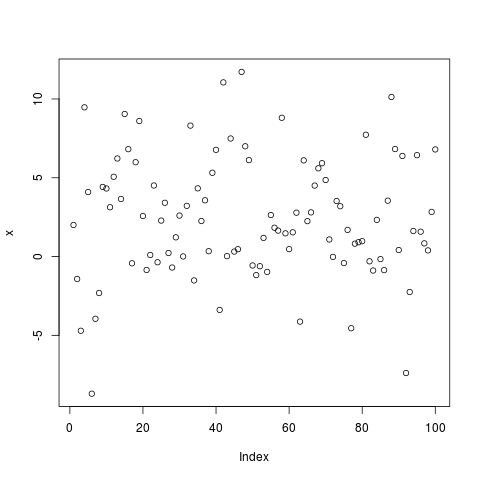
\includegraphics[width=4cm]{plot1.png}}{plot1.png}
\end{center}
\end{itemize}
\end{frame}

\begin{frame}\frametitle{Nothing is lost or hidden}
  \begin{itemize}
    \item statistical packages provide \emph{canned} procedures to address common statistical problems
    \item canned procedures are useful for routine analysis, but they are also limiting - you can only do what the programmer lets you do 
    \item in R, the result of statistical calculation are always accessible, so
      \begin{itemize}
        \item you can use them for further calculations
        \item you can always see how calculations were done
      \end{itemize}
    \item what you see in the first place is most of the time only a small part of the result
  \end{itemize}
\end{frame}


\begin{frame}[fragile]\frametitle{Nothing is lost or hidden}
\begin{itemize}
\item for example building a linear model gives you the following result
\begin{semiverbatim}
> lm(y~x)

Call:
lm(formula = y ~ x)

Coefficients:
(Intercept)            x  
    0.07101      1.98083  
\end{semiverbatim}
\end{itemize}
\end{frame}


\begin{frame}[fragile]\frametitle{Nothing is lost or hidden}
\begin{itemize}
\item save the model in an object mm so you can run functions on it, e.g. \texttt{summary()} or \texttt{plot()}
\scriptsize
\begin{semiverbatim}
> mm <- lm(y~x)
> summary(mm)

Call:
lm(formula = y ~ x)

Residuals:
     Min       1Q   Median       3Q      Max 
-1.67162 -0.36329  0.02206  0.29193  1.36333 

Coefficients:
            Estimate Std. Error t value Pr(>|t|)    
(Intercept)  0.07101    0.06353   1.118    0.266    
x            1.98083    0.01404 141.043   <2e-16 ***
---
Signif. codes:  0 ‘***’ 0.001 ‘**’ 0.01 ‘*’ 0.05 ‘.’ 0.1 ‘ ’ 1

Residual standard error: 0.5385 on 98 degrees of freedom
Multiple R-squared:  0.9951,	Adjusted R-squared:  0.995 
F-statistic: 1.989e+04 on 1 and 98 DF,  p-value: < 2.2e-16
\end{semiverbatim}
\end{itemize}
\end{frame}


\begin{frame}[fragile]\frametitle{Nothing is lost or hidden}
\begin{itemize}
\item to explore the object you can use the object browser or \texttt{str()}
\scriptsize
\begin{semiverbatim}
> str(mm)
List of 12
 $ coefficients : Named num [1:2] 0.071 1.981
  ..- attr(*, "names")= chr [1:2] "(Intercept)" "x"
 $ residuals    : Named num [1:100] 0.6828 -0.1417 0.0992 0.1057 ...
  ..- attr(*, "names")= chr [1:100] "1" "2" "3" "4" ...
 $ effects      : Named num [1:100] -48.23926 -75.95182 0.04414 ...
  ..- attr(*, "names")= chr [1:100] "(Intercept)" "x" "" "" ...
 $ rank         : int 2
 $ fitted.values: Named num [1:100] 9.18 13.41 8.12 15.11 5.96 ...
  ..- attr(*, "names")= chr [1:100] "1" "2" "3" "4" ...
 $ assign       : int [1:2] 0 1
 $ qr           :List of 5
  ..$ qr   : num [1:100, 1:2] -10 0.1 0.1 0.1 0.1 0.1 0.1  ...
  .. ..- attr(*, "dimnames")=List of 2
  .. .. ..$ : chr [1:100] "1" "2" "3" "4" ...
  .. .. ..$ : chr [1:2] "(Intercept)" "x"
  .. ..- attr(*, "assign")= int [1:2] 0 1
...
\end{semiverbatim}
\end{itemize}
\end{frame}


\subsection{Help}
\begin{frame}[fragile]\frametitle{First Session}
\begin{itemize}
\item Entering the command
\begin{verbatim}
 > help.start()
\end{verbatim}
at the command line, will launch an extensive online help that can be read using a Web browser such as Firefox or Internet Explorer. Another way to access to these ''help'' pages is the help tab in the bottom right corner. Notice that the HTML version of the help system has a very useful ''Search Engine and Keywords''.
\end{itemize}
\end{frame}


\begin{frame}[fragile]\frametitle{First Session}
\begin{center}
  \linkimage{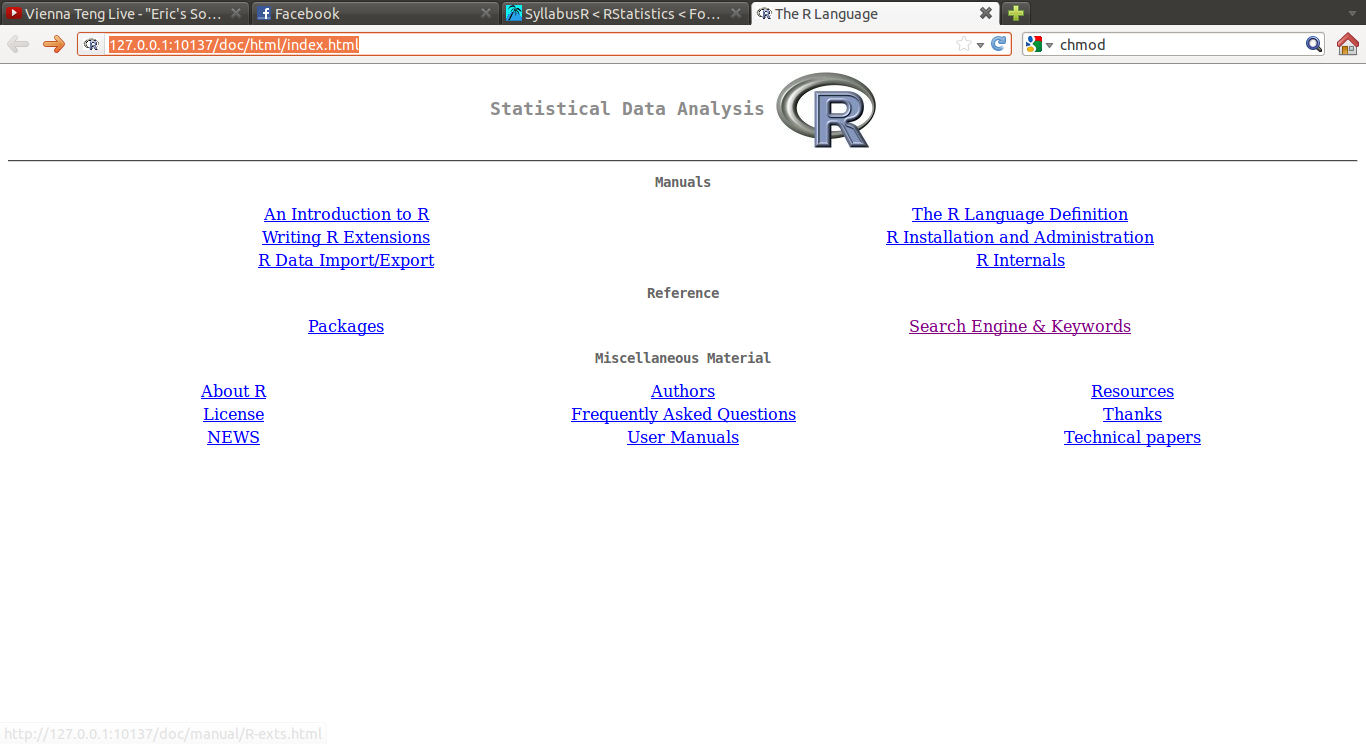
\includegraphics[width=11cm]{help.png}}{help.png}
\end{center}
\end{frame}



\subsection{Quitting}
\begin{frame}[fragile]\frametitle{First Session}
\begin{itemize}
\item All variables, functions and diverse objects can be seen by the \texttt{ls()} and the newer version of it \texttt{objects()} function. Thus in our example we will have
\begin{semiverbatim}
> ls()
[1] "x"
\end{semiverbatim}
\item quitting R is done with the  \texttt{q()} function
\begin{semiverbatim}
> q()
\end{semiverbatim}
at the command prompt. You will be asked to save your ''workspace image''. Give a name for your workspace for example ''project1''.

\item you can load this workspace in a new R session. On windows just click directly on the workspace file and R will be opened and automatically load the workspace
\end{itemize}
\end{frame}



\section{Citation/License}
\subsection{Citation}
\begin{frame}[shrink=11,fragile,c]\frametitle{Citation}
  \begin{block}{Input}
\begin{semiverbatim}
> citation()
\end{semiverbatim}
  \end{block}
\begin{semiverbatim}
To cite R in publications use:

  R Development Core Team (2012). R: A language and environment for
  statistical computing. R Foundation for Statistical Computing,
  Vienna, Austria. ISBN 3-900051-07-0, URL http://www.R-project.org/.

A BibTeX entry for LaTeX users is

  @Manual{,
    title = {R: A Language and Environment for Statistical Computing},
    author = {{R Development Core Team}},
    organization = {R Foundation for Statistical Computing},
    address = {Vienna, Austria},
    year = {2012},
    note = {{ISBN} 3-900051-07-0},
    url = {http://www.R-project.org/},
  }

We have invested a lot of time and effort in creating R, please cite it
when using it for data analysis. See also ‘citation("pkgname")’ for
citing R packages.

\end{semiverbatim}
\end{frame}

\subsection{License}
\begin{frame}\frametitle{Licence}
\begin{alertblock}{Licence}
R is mainly distributed under the terms of the GNU General
Public License, either Version 2, June 1991 or Version 3, June 2007. Core Bioconductor packages are typically licensed under Artistic-2.0. You get detailed information with: \texttt{license(), RShowDoc("COPYING"), packageDescription("packagename")\$License}
\end{alertblock}
\end{frame}

\appendix
\flushlinkimages

\end{document}
